\documentclass[a4paper, 10pt]{article}

%% Language and font encodings
\usepackage[english]{babel}
\usepackage[utf8]{inputenc}
\usepackage[T1]{fontenc}

%% Sets page size and margins
\usepackage[a4paper,top=2.5cm,bottom=2.3cm,left=2.5cm,right=1.9cm]{geometry}


%% Useful packages
\usepackage{amsmath}
\usepackage{siunitx}
\usepackage{booktabs}
\usepackage{graphicx}
\usepackage[colorinlistoftodos]{todonotes}
\usepackage[colorlinks=true, allcolors=blue]{hyperref}
\usepackage{hyperref}
\usepackage{subcaption}
\usepackage{multirow}
\usepackage{arydshln}  % dashed lines
\usepackage{changepage}
\usepackage{blindtext} % lorem ipsum

\renewcommand{\arraystretch}{1.25} % for tables

\title{Your Paper}
\author{You}

\begin{document}
\maketitle
\newpage
\section{Lab 1}
\subsection{Algorithm comparison}
  \begin{table}[h!]
    \begin{tabular}{@{}lrrrr@{}}
      \toprule
      \multicolumn{5}{c}{\textbf{gd}} \\
      N  &   $R_t$  &  $MSE_t$ &  Epch  & T(s)\\
      \midrule
      10       &   0.06     &  0.49       &  771     & 2.64   \\
      20       &   0.31     &  0.37       &  849     & 2.82   \\
      40       &   0.32     &  0.35       &  915     & 3.58   \\
      80       &   0.49     &  0.27       &  958     & 4.12   \\
      \hdashline
      100      &   0.48     &  0.53       &  976     & 4.90   \\
      120      &   0.47     &  0.62       &  957     & 7.15   \\
      \bottomrule
    \end{tabular} 
    \hfill
    \begin{tabular}{@{}lrrrr@{}}
      \toprule
      \multicolumn{5}{c}{\textbf{gda}} \\
      N  &   $R_t$  &  $MSE_t$ &  Epch  & T(s)\\
      \midrule
      10  & 0.17    & 0.51    & 79      &  0.28   \\
      20  & 0.25    & 0.48    & 79      &  0.53   \\
      40  & 0.29    & 0.54    & 67      &  0.58   \\
      80  & 0.22    & 0.88    & 68      &  0.59   \\                 
      \hdashline
      100 & 0.20    & 0.90    & 112     &  0.51   \\
      120 & 0.21    & 1.15    & 97      &  0.47   \\
      \bottomrule
    \end{tabular} 
    \hfill
    \begin{tabular}{@{}lrrrr@{}}
      \toprule
      \multicolumn{5}{c}{\textbf{cgf}} \\
      N  &   $R_t$  &  $MSE_t$ &  Epch  & T(s)\\
      \midrule
      10  & 0.15    & 0.50    & 11      &  0.10  \\
      20  & 0.42    & 0.38    & 17      &  0.31  \\
      40  & 0.65    & 0.28    & 30      &  0.54  \\
      80  & 0.69    & 0.29    & 44      &  0.53  \\
      \hdashline
     100  & 0.68    & 0.35    & 37      &  0.59  \\
     120  & 0.60    & 0.45    & 38      &  0.76  \\
      \bottomrule
    \end{tabular} 
    \mbox{}
    \begin{tabular}{@{}lrrrr@{}}
      \toprule
      \multicolumn{5}{c}{\textbf{cgp}} \\
      N  &   $R_t$  &  $MSE_t$ &  Epch  & T(s)\\
      \midrule
      10  & 0.17    & 0.48    & 12      &  0.10  \\
      20  & 0.33    & 0.48    & 15      &  0.40  \\
      40  & 0.60    & 0.32    & 25      &  0.48  \\
      80  & 0.67    & 0.31    & 35      &  1.59  \\
      \hdashline
     100  & 0.62    & 0.38    & 40      &  0.66  \\
     120  & 0.62    & 0.44    & 32      &  0.63  \\
      \bottomrule
    \end{tabular} 
    \hfill
    \begin{tabular}{@{}lrrrr@{}}
      \toprule
      \multicolumn{5}{c}{\textbf{bfg}} \\
      N  &   $R_t$  &  $MSE_t$ &  Epch  & T(s)\\
      \midrule
      10  & 0.18    & 0.48   & 11       & 0.15  \\
      20  & 0.43    & 0.40   & 17       & 0.30  \\
      40  & 0.77    & 0.20   & 35       & 0.86  \\
      80  & 0.91    & 0.9    & 39       & 2.34  \\
      \hdashline
     100  & 0.88    & 0.12   & 47       & 2.55  \\   
     120  & 0.75    & 0.28   & 47       & 3.59  \\
      \bottomrule
    \end{tabular} 
    \hfill
    \begin{tabular}{@{}lrrrr@{}}
      \toprule
      \multicolumn{5}{c}{\textbf{lm}} \\
      N  &   $R_t$  &  $MSE_t$ &  Epch  & T(s)\\
      \midrule
      10  & 0.18    & 0.44   & 11       & 0.07  \\ 
      20  & 0.50    & 0.38   &  6       & 0.10  \\ 
      40  & 0.85    & 0.13   & 11       & 0.18  \\ 
      \textbf{80} & \textbf{.93} & \textbf{.07}  & \textbf{6} & \textbf{.31} \\
      \hdashline
     100  & 0.90    & 0.10   & 4        & 0.26  \\
     120  & 0.81    & 0.22   & 5        & 0.27  \\  
      \bottomrule
    \end{tabular} \mbox{}
    \caption{Performance of different training algorithms. Results are the
      average ones after twenty runs on the test set. \emph{N} is the
      neurons on the hidden layer. $R_t$ and $MSE_t$ 
    stand for regression R-value and for MSE on the test set, respectively. 
    Test size is 15\% of the total data. \emph{Epch} stands for epoch of 
    convergence. \emph{T(s)} is time (seconds). Best result is 
    highlighted in bold. The dotted line separates overfitted results}
    \label{tab:train_algs}
  \end{table}

  \begin{figure}[h]
    \begin{adjustwidth}{-1.1cm}{-1.1cm}
    \centering
    \begin{subfigure}[t]{0.3\linewidth}
      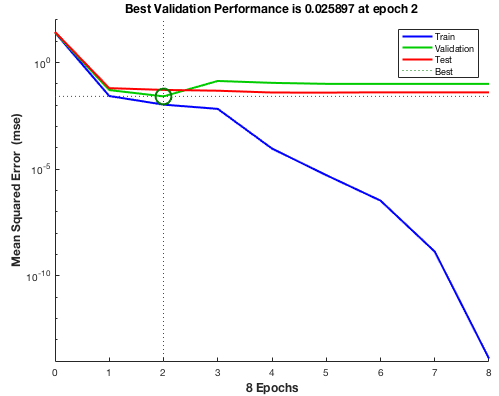
\includegraphics[width=1\linewidth]{./lab1/overfit_stop.png}
      \caption{Validation set avoids overfitting}
      \label{fig:perfect_fit}
    \end{subfigure}
    \begin{subfigure}[t]{0.3\linewidth}
      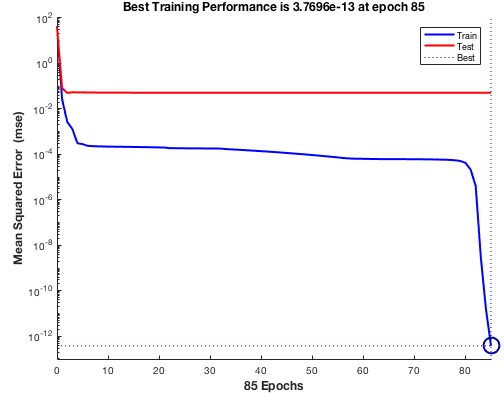
\includegraphics[width=1\linewidth]{./lab1/overfit.png}
      \caption{Overfit. 120 Neurons}
      \label{fig:overfit}
    \end{subfigure}
    \begin{subfigure}[t]{0.3\linewidth}
      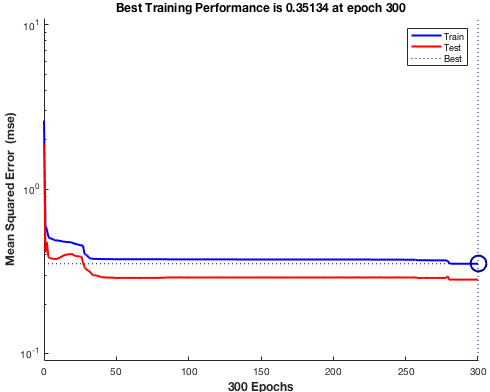
\includegraphics[width=1\linewidth]{./lab1/underfit.png}
      \caption{Underfit. 5 Neurons}
      \label{fig:underfit}
    \end{subfigure}
    \end{adjustwidth}
    \caption{Evolution of test (red), train (blue) and validation (green) set 
      MSE during training.  Left figure uses a validation set that stops befor
      e overfitting.  Otherwise, train error keeps sinking after the optima, a
      s \autoref{fig:overfit} also shows. On the right, with 5 neurons, the 
      training never converges: the net is too simple to learn the function, 
      error never decays. Test error (red) is lower than training error, it
      underfits.}
    \label{fig:validation}
  \end{figure}


  The goal here is comparing the six algorithms for training Neural Nets on
  the Matlab toolbox. For this purpose, I have trained a net using each 
  algorithm with different number of hidden units. Then, I have evaluated
  is performance on the test set, and repeated the process twenty times. 
  \autoref{tab:train_algs} shows the results of these experiments, averaged for
  each algorithm and neuron setting. Overall, all algorithms perform best
  with 80 hidden units: nets with neurons over that threshold 
  are overparametrized, since their MSE on the test set starts to decrease. 
  If there was no validation set, for 100 and 120 neurons the MSE on 
  train set would be way higher than that of test set, as
  \autoref{fig:validation} shows. On the other hand, nets with few hidden units
  do not even learn the model, and can have higher train error than test, as in
  \autoref{fig:underfit}.

  The best algorithm
  in terms of speed and performance is the \emph{Levenberg-Marquardt} (lm)
  algorithm: it trains the fastest and it reaches better performance
  than the other ones under the same configurations. \emph{Gradient descent}
  is by far the worst, both in speed and accuracy. The reason is that [maybe 
  that looks for the best option/not optimized -check]

  \subsubsection{Noisy data}
    \begin{figure}[h]
      \begin{adjustwidth}{-1.1cm}{-1.1cm}
      \centering
      \begin{subfigure}[t]{0.31\linewidth}
        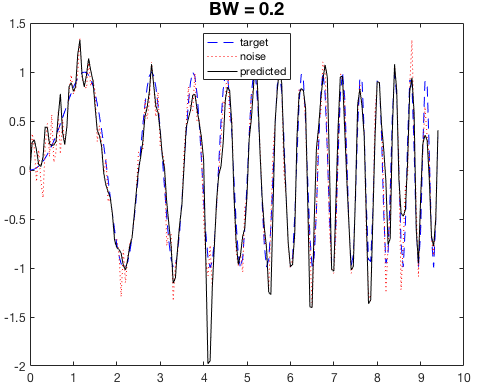
\includegraphics[width=1\linewidth]{./lab1/noise_2e-1.png}
        \caption{$R_t=0.54$, $MSE_t=0.53$}
        \label{fig:noise_small}
      \end{subfigure}
      \begin{subfigure}[t]{0.30\linewidth}
        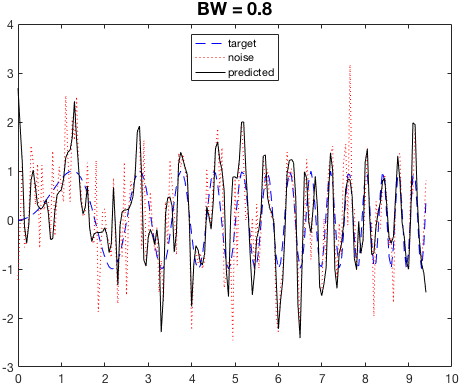
\includegraphics[width=1\linewidth]{./lab1/noise_8e-1.png}
        \caption{$R_t=0.38$, $MSE_t=2.25$}
        \label{fig:noise_big}
      \end{subfigure}
      \begin{subfigure}[t]{0.3\linewidth}
        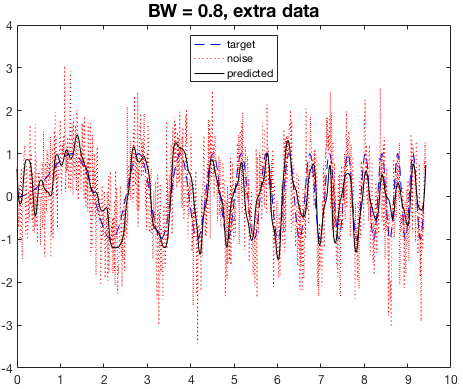
\includegraphics[width=1\linewidth]{./lab1/noise_8e-1_extra.png}
        \caption{$R_t=0.58$, $MSE_t=0.82$}
        \label{fig:noise_more_data}
      \end{subfigure}
      \end{adjustwidth}
      \caption{Estimation of a function with Gaussian noise, 0 mean, and different
        $\sigma$, or \emph{BW}. Figures (a) and (b) estimate on 190 data points, 
        figure (c) estimates on 950, 5 times more points. The network contains 80 
        hidden units, and it was trained using the \emph{lm} algorithm. MSE 
        with noisy data is worse, compared with the same setup on 
        \autoref{tab:train_algs}. Increasing the data points reduces again the 
        error, as (c) shows.}
      \label{fig:noise}
    \end{figure}

\subsection{Bayesian Inference}
  \begin{figure}[h]
    \centering
    \hfill
    \begin{tabular}{@{}lrrrrr@{}}
      \toprule
      \multicolumn{6}{c}{\textbf{Levenberg-Marquardt}} \\
      N  &   $R_t$  &  $MSE_t$ &  $MSE_{tr}$ & Epch  & T(s)\\
      \midrule
      50   &   0.97    &   0.03    &  \num{0.81d-2}  &  8   &  0.15  \\
      100  &   0.90    &   0.10    &  \num{0.29d-2}  &  6   &  0.33  \\
      150  &   0.76    &   0.28    &  \num{0.01d-2}  &  5   &  0.31  \\
      300  &   0.41    &   1.00    &  \num{0.27d-2}  &  3   &  1.28  \\
      \bottomrule
    \end{tabular} 
    \hfill
    \begin{tabular}{@{}lrrrrr@{}}
      \toprule
      \multicolumn{6}{c}{\textbf{Bayesian Optimization}} \\
      N  &   $R_t$  &  $MSE_t$ & $MSE_{tr}$  & Epch  & T(s)\\
      \midrule
      50   &   1.00    &   \num{d-4}  &  \num{0.94d-7}   & 150   &    2.11  \\
      100  &   0.98    &   0.02       &  \num{0.50d-2}   & 106   &    6.52  \\
      150  &   0.89    &   0.11       &  \num{0.22d-4}   &  33   &   13.69  \\
      300  &   0.61    &   0.62       &  \num{0.19d-7}   &  27   &   92.65  \\
      \bottomrule
    \end{tabular}  \hfill\mbox{}
    \caption{}
    \label{fig:bayes}
  \end{figure}

  





\newpage
\section{Unsupervised Learning}
  \subsection{Principal Component Analysis}
  The goal of this section is to understand the meaning and consequences of using
  PCA, applied to the \emph{threes} dataset. \autoref{fig:first_task} summarizes the data:
  on the right I present the average \emph{three}, on the left the eigenvalues, 
  scaled over their sum. The first components explain most of the variance:
  just 12 explain 63\%, and with 50 it adds up to 90\%. Therefore, 50 components 
  should already deliver a good reconstruction of the data. The right panel
  of \autoref{fig:many_pc} proves it; with 64 and 128 PC the result
  is almost the original sample. With 256 PC the recovered image is exactly
  the same, and the \emph{MSE} is 0. With data $X \in {\rm I\!R}^{d \times N}$,
  being $d$ the input feature space; $V \in {\rm I\!R}^{d \times s}$ the
  eigenvector matrix, $s$ selected components; and $X_s=V^{t}X$ the data
  projected on those components. If $s=d$, then $VV^{t}=I$ (full rank orthogonal matrix).
  Then, $\hat{X} = VX_s = VV^{t}X = X$. 
  
  \begin{figure}[h]
    \centering
    \begin{subfigure}[t]{0.4\linewidth}
      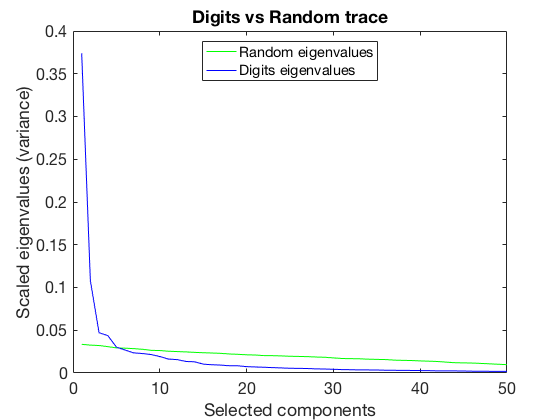
\includegraphics[width=1\linewidth]{./lab3/PCA/digits_vs_random_trace.png}
      \label{fig:trace_compared}
    \end{subfigure}
    \begin{subfigure}[t]{0.3\linewidth}
      
\includegraphics[width=1\linewidth, height=4.75cm]{./lab3/PCA/mean_three.png}
      \label{fig:mean_three}
    \end{subfigure}
    \caption{First task of the exercise: computing the mean three (right), and 
    plotting the first 50 eigenvalues (left). They have been compared
  to those of a random, multivariate Gaussian distribution, in green.}
    \label{fig:first_task}
  \end{figure}

  \begin{figure}[h]
    \centering
    \begin{subfigure}[t]{0.49\linewidth}
      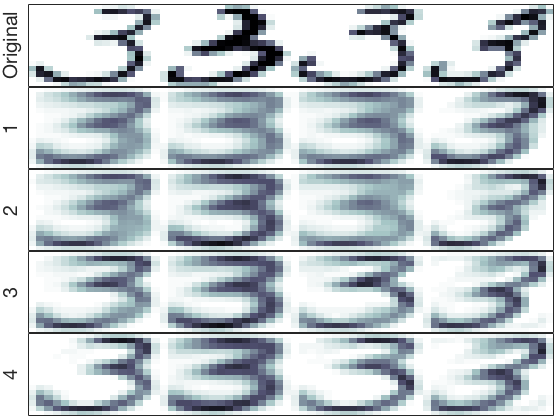
\includegraphics[width=1\linewidth]{./lab3/PCA/mosaics/PC_1_4_small.png}
      \caption{Few PC. $MSE(rec) > 0.9; variance < 12\%$}
      \label{fig:few_pc}
    \end{subfigure}
    \begin{subfigure}[t]{0.49\linewidth}
      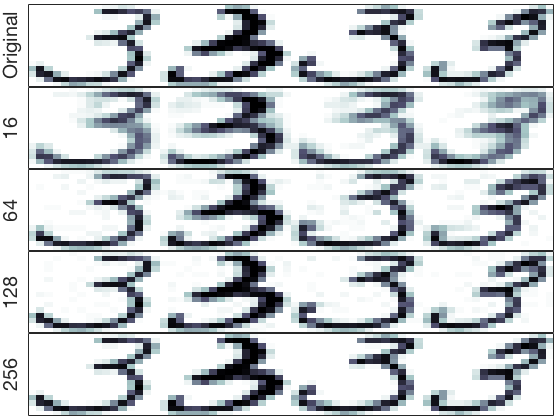
\includegraphics[width=1\linewidth]{./lab3/PCA/mosaics/PC_16_256_small.png}
      \caption{Many PC. $MSE(rec) < 0.75; variance > 45\%$}
      \label{fig:many_pc}
    \end{subfigure}
    \caption{Reconstruction of four different samples (columns) with increasing
      number of components (rows). Top row of each table contains the 
    original samples. Vertical labels indicate the number of components}
    \label{fig:threes_pc}
  \end{figure}

  With Gaussian data 50 components are not enough: they explain only 43\% of the 
  variance, and deliver a reconstruction error of 0.77 (\autoref{fig:gauss_rec}),
  whereas in the digits it is already below 0.1 (\autoref{fig:digits_rec}). 
  It makes sense, because in random data all features carry the same variance, 
  there is no optimal direction.  Therefore, the eigenvalues sink more gradually,
  as in \autoref{fig:first_task}.  Anyway, both datasets show a strong 
  correlation between the sum of variance of the last $k$ left-out components 
  and the reconstruction $MSE$, displayed in \autoref{fig:regression}. The shape
  of the curve suggests that the relationship between them is logarithmic, 
  rather than linear.

  \begin{figure}[h]
    \begin{adjustwidth}{-1cm}{-1cm}
    \centering
    \begin{subfigure}[t]{0.3\linewidth}
      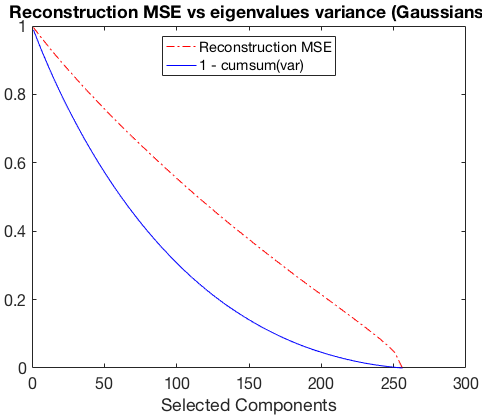
\includegraphics[width=1\linewidth]{./lab3/PCA/rec_vs_invsum_gauss.png}
      \caption{Gaussians dataset}
      \label{fig:gauss_rec}
    \end{subfigure}
    \begin{subfigure}[t]{0.3\linewidth}
      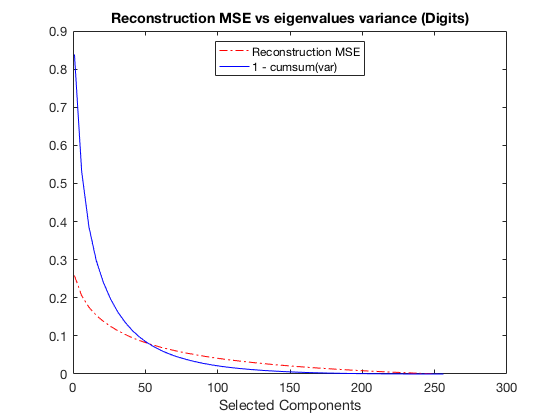
\includegraphics[width=1\linewidth, height=4.7cm]{./lab3/PCA/rec_vs_invsum_digits.png}
      \caption{Digits dataset}
      \label{fig:digits_rec}
    \end{subfigure}
    \begin{subfigure}[t]{0.3\linewidth}
      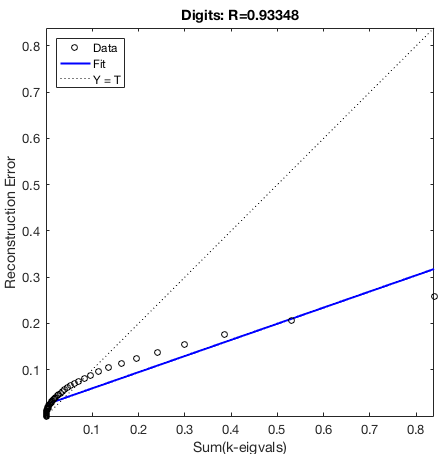
\includegraphics[width=1\linewidth, height=4.7cm]{./lab3/PCA/regression_digits.png}
      \caption{Reconstruction MSE linear fit}
      \label{fig:regression}
    \end{subfigure}
    \end{adjustwidth}
    \caption{Plot of the reconstruction $MSE$ for each number of selected $k$ components (red),
    against the sum of the variance of the last $256-k$ components (blue), on 
  different datasets. Right figure plots their linear fit.}
    \label{fig:rec_vs_cumsum}
  \end{figure}
  

  % still needs improvement. If I cannot expand the pages and add the
  % components interpretation, put this (model the main structure of the data)
  % in the threes footnote, and remove this paragraph
  \paragraph{Visual interpretation} a sample with few components 
  if much different from the original image, as the images on \autoref{fig:few_pc} 
  show. These recovered images seem more similar to the average \emph{three} of 
  \autoref{fig:first_task}. The reason is that the first components model the
  main structure underlying all the data, the \emph{essence} of the \emph{threes}.
  As more components are added, reconstruction becomes more accurate.  The last 
  components model the noise, the particularities of each data point. Since
  most variance lies below 50 PC, any reconstruction with more than those delivers
  almost the same result, as seen on \autoref{fig:many_pc}
  

  \begin{figure}[h]
    \centering
    \begin{subfigure}[t]{0.16\linewidth}
      
\includegraphics[width=1\linewidth]{./lab3/PCA/PC_interpret/PC1.png}
      \caption{PC 1}
      \label{fig:PC1}
    \end{subfigure}
    \begin{subfigure}[t]{0.16\linewidth}
      
\includegraphics[width=1\linewidth]{./lab3/PCA/PC_interpret/PC1_02.png}
      \caption{0.2}
      \label{fig:quant02}
    \end{subfigure}
    \begin{subfigure}[t]{0.16\linewidth}
      
\includegraphics[width=1\linewidth]{./lab3/PCA/PC_interpret/PC1_04.png}
      \caption{0.4}
      \label{fig:quant04}
    \end{subfigure}
    \begin{subfigure}[t]{0.16\linewidth}
      
\includegraphics[width=1\linewidth]{./lab3/PCA/PC_interpret/PC1_06.png}
      \caption{0.6}
      \label{fig:quant06}
    \end{subfigure}
    \begin{subfigure}[t]{0.16\linewidth}
      
\includegraphics[width=1\linewidth]{./lab3/PCA/PC_interpret/PC1_08.png}
      \caption{0.8}
      \label{fig:quant08}
    \end{subfigure}
    \begin{subfigure}[t]{0.16\linewidth}
      
\includegraphics[width=1\linewidth]{./lab3/PCA/PC_interpret/PC1_1.png}
      \caption{1}
      \label{fig:quant1}
    \end{subfigure}
    \caption{First principal component plotted (left) along with threes corresponding
    to different quantiles, on the data distribution over that PC. Quantile below
  the image}
    \label{fig:quantiles}
  \end{figure}




  \subsection{Self Organizing Map}
  %https://nl.mathworks.com/help/nnet/ug/cluster-with-self-organizing-map-neural-network.html
  \Blindtext



  \begin{figure}[h]
    \centering
    \hfill
    \begin{tabular}{@{}rcrrrcrrrcrrr@{}}
      \toprule
      \multicolumn{1}{l}{\multirow{2}{*}{$Iterations$}} & \phantom{a} &% fake multicolumn alligns mulitrow
        \multicolumn{3}{c}{\textbf{Hexagonal topology}} & \phantom{a} &
        \multicolumn{3}{c}{\textbf{Grid topology}}      & \phantom{a} &
        \multicolumn{3}{c}{\textbf{Random topology}} \\
      \cmidrule{3-5} \cmidrule{7-9} \cmidrule{11-13}
      && Link & Euc. & Box && Link & Euc. & Box && Link & Euc. & Box  \\
      \midrule
      $initHood = 3$ \\
      \emph{100}  &&  0.7240  &  0.7274  &  0.7247  &&  0.7261  &  0.7240  &  0.7212  &&  0.6934  &  0.6799  &  0.6492 \\
      %\emph{150}  &&  0.7240  &  0.7219  &  0.7240  &&  0.7247  &  0.7219  &  0.7219  &&  0.6792  &  0.6522  &  0.6214 \\
      \emph{200}  &&  0.7275  &  0.7239  &  0.7247  &&  0.7268  &  0.7246  &  0.7240  &&  0.6940  &  0.6225  &  0.6210 \\
      %\emph{250}  &&  0.7233  &  0.7240  &  0.7226  &&  0.7232  &  0.7275  &  0.7233  &&  0.7253  &  0.6497  &  0.5628 \\
      \emph{300}  &&  0.7275  &  0.7253  &  0.7260  &&  0.7219  &  0.7219  &  0.7261  &&  0.7096  &  0.6489  &  0.6083 \\
      %\emph{350}  &&  0.7212  &  0.7240  &  0.7212  &&  0.7254  &  0.7212  &  0.7247  &&  0.7226  &  0.6081  &  0.5631 \\
      \emph{400}  &&  0.7212  &  0.7232  &  0.7233  &&  0.7240  &  0.7240  &  0.7247  &&  0.7126  &  0.6051  &  0.6660 \\
      %\emph{450}  &&  0.7233  &  0.7226  &  0.7240  &&  0.7254  &  0.7268  &  0.7253  &&  0.6827  &  0.5925  &  0.5917 \\
      \emph{500}  &&  0.7261  &  0.7240  &  0.7254  &&  0.7233  &  0.7240  &  0.7253  &&  0.7226  &  0.6214  &  0.6061 \\
      $initHood = 4$ \\
      \emph{100}  &&  0.7219  &  0.7232  &  0.7219  &&  0.7247  &  0.7254  &  0.7240  &&  0.6815  &  0.6366  &  0.6518 \\
      %\emph{150}  &&  0.7232  &  0.7247  &  0.7254  &&  0.7261  &  0.7247  &  0.7233  &&  0.6815  &  0.6506  &  0.6221 \\
      \emph{200}  &&  0.7239  &  0.7240  &  0.7240  &&  0.7267  &  0.7205  &  0.7240  &&  0.6942  &  0.6379  &  0.6355 \\
      %\emph{250}  &&  0.7247  &  0.7282  &  0.7233  &&  0.7233  &  0.7247  &  0.7254  &&  0.7226  &  0.5920  &  0.6504 \\
      \emph{300}  &&  0.7233  &  0.7240  &  0.7240  &&  0.7261  &  0.7219  &  0.7233  &&  0.7233  &  0.6351  &  0.6499 \\
      %\emph{350}  &&  0.7226  &  0.7247  &  0.7247  &&  0.7254  &  0.7233  &  0.7240  &&  0.7101  &  0.6213  &  0.6066 \\
      \emph{400}  &&  0.7240  &  0.7239  &  0.7246  &&  0.7233  &  0.7254  &  0.7233  &&  0.6801  &  0.6055  &  0.5944 \\
      %\emph{450}  &&  0.7226  &  0.7240  &  0.7261  &&  0.7254  &  0.7275  &  0.7233  &&  0.7239  &  0.6071  &  0.6090 \\
      \emph{500}  &&  0.7226  &  0.7232  &  0.7261  &&  0.7233  &  0.7219  &  0.7226  &&  0.7112  &  0.6081  &  0.6047 \\
      $initHood = 5$ \\
      \emph{100}  &&  0.7233  &  0.7247  &  0.7219  &&  0.7240  &  0.7233  &  0.7240  &&  0.6963  &  0.7121  &  0.6512 \\
      %\emph{150}  &&  0.7240  &  0.7233  &  0.7212  &&  0.7247  &  0.7253  &  0.7247  &&  0.7240  &  0.6626  &  0.6357 \\
      \emph{200}  &&  0.7254  &  0.7225  &  0.7254  &&  0.7247  &  0.7247  &  0.7275  &&  0.7079  &  0.6062  &  0.6524 \\
      %\emph{250}  &&  0.7261  &  0.7226  &  0.7246  &&  0.7239  &  0.7233  &  0.7226  &&  0.7121  &  0.6229  &  0.6485 \\
      \emph{300}  &&  0.7239  &  0.7233  &  0.7219  &&  0.7233  &  0.7260  &  0.7254  &&  0.7103  &  0.5344  &  0.5914 \\
      %\emph{350}  &&  0.7246  &  0.7240  &  0.7247  &&  0.7240  &  0.7233  &  0.7247  &&  0.6940  &  0.6525  &  0.6510 \\
      \emph{400}  &&  0.7240  &  0.7261  &  0.7240  &&  0.7240  &  0.7261  &  0.7219  &&  0.6935  &  0.6496  &  0.6532 \\
      %\emph{450}  &&  0.7261  &  0.7275  &  0.7232  &&  0.7219  &  0.7233  &  0.7219  &&  0.7091  &  0.6560  &  0.6344 \\
      \emph{500}  &&  0.7261  &  0.7226  &  0.7240  &&  0.7226  &  0.7233  &  0.7226  &&  0.6954  &  0.6041  &  0.5914 \\
      $initHood = 50$ \\
      \emph{100}  &&  0.7254  &  0.7240  &  0.7247  &&  0.7226  &  0.7239  &  0.7226  &&  0.7240  &  0.7240  &  0.7246 \\
      %\emph{150}  &&  0.7219  &  0.7247  &  0.7219  &&  0.7261  &  0.7268  &  0.7233  &&  0.7226  &  0.7261  &  0.7268 \\
      \emph{200}  &&  0.7240  &  0.7240  &  0.7247  &&  0.7226  &  0.7240  &  0.7199  &&  0.6639  &  0.7205  &  0.7212 \\
      %\emph{250}  &&  0.7239  &  0.7233  &  0.7233  &&  0.7253  &  0.7219  &  0.7212  &&  0.7084  &  0.7068  &  0.7240 \\
      \emph{300}  &&  0.7247  &  0.7240  &  0.7260  &&  0.7233  &  0.7261  &  0.7247  &&  0.7103  &  0.7212  &  0.7213 \\
      %\emph{350}  &&  0.7226  &  0.7268  &  0.7261  &&  0.7268  &  0.7240  &  0.7247  &&  0.7112  &  0.7247  &  0.7212 \\
      \emph{400}  &&  0.7240  &  0.7247  &  0.7247  &&  0.7254  &  0.7240  &  0.7240  &&  0.7070  &  0.7070  &  0.7240 \\
      %\emph{450}  &&  0.7219  &  0.7254  &  0.7233  &&  0.7253  &  0.7233  &  0.7212  &&  0.7103  &  0.7112  &  0.7077 \\
      \emph{500}  &&  0.7226  &  0.7226  &  0.7254  &&  0.7226  &  0.7240  &  0.7282  &&  0.7091  &  0.7226  &  0.7091 \\
        %$initHood = 100$ \\
%        ARI_matrix(:,:,1) =
%
%    0.7254    0.7275    0.7198
%    0.7219    0.7254    0.7261
%    0.7233    0.7260    0.7240
%    0.7254    0.7253    0.7240
%    0.7239    0.7219    0.7233
%    0.7253    0.7240    0.7254
%    0.7240    0.7219    0.7247
%    0.7247    0.7226    0.7261
%    0.7260    0.7233    0.7233
%
%
%ARI_matrix(:,:,2) =
%
%    0.7233    0.7247    0.7246
%    0.7219    0.7240    0.7253
%    0.7233    0.7226    0.7247
%    0.7254    0.7205    0.7240
%    0.7233    0.7233    0.7282
%    0.7232    0.7254    0.7268
%    0.7233    0.7253    0.7247
%    0.7240    0.7219    0.7261
%    0.7247    0.7233    0.7253
         \bottomrule
      \end{tabular} 
      \caption{}
      \label{fig:bayes}
    \end{figure}




    
    
    
    
    
    
    
    
    
\end{document}

